MeReader follows a component-based architecture focusing on the separation of concerns and modularity. This approach allows individual components of the system to be developed, tested, and maintained independently, thereby reducing the risk of introducing regressions or conflicts in the core functionality during system evolution. It also facilitates easier scaling and integration of new features, ensuring that future enhancements can be incorporated with minimal disruption to the existing codebase. The design of MeReader integrates principles from both object-oriented programming (OOP) and service-oriented (SOA) architecture to establish robust and well-defined boundaries between system components.

\begin{figure}[!htbp]
  \centering
  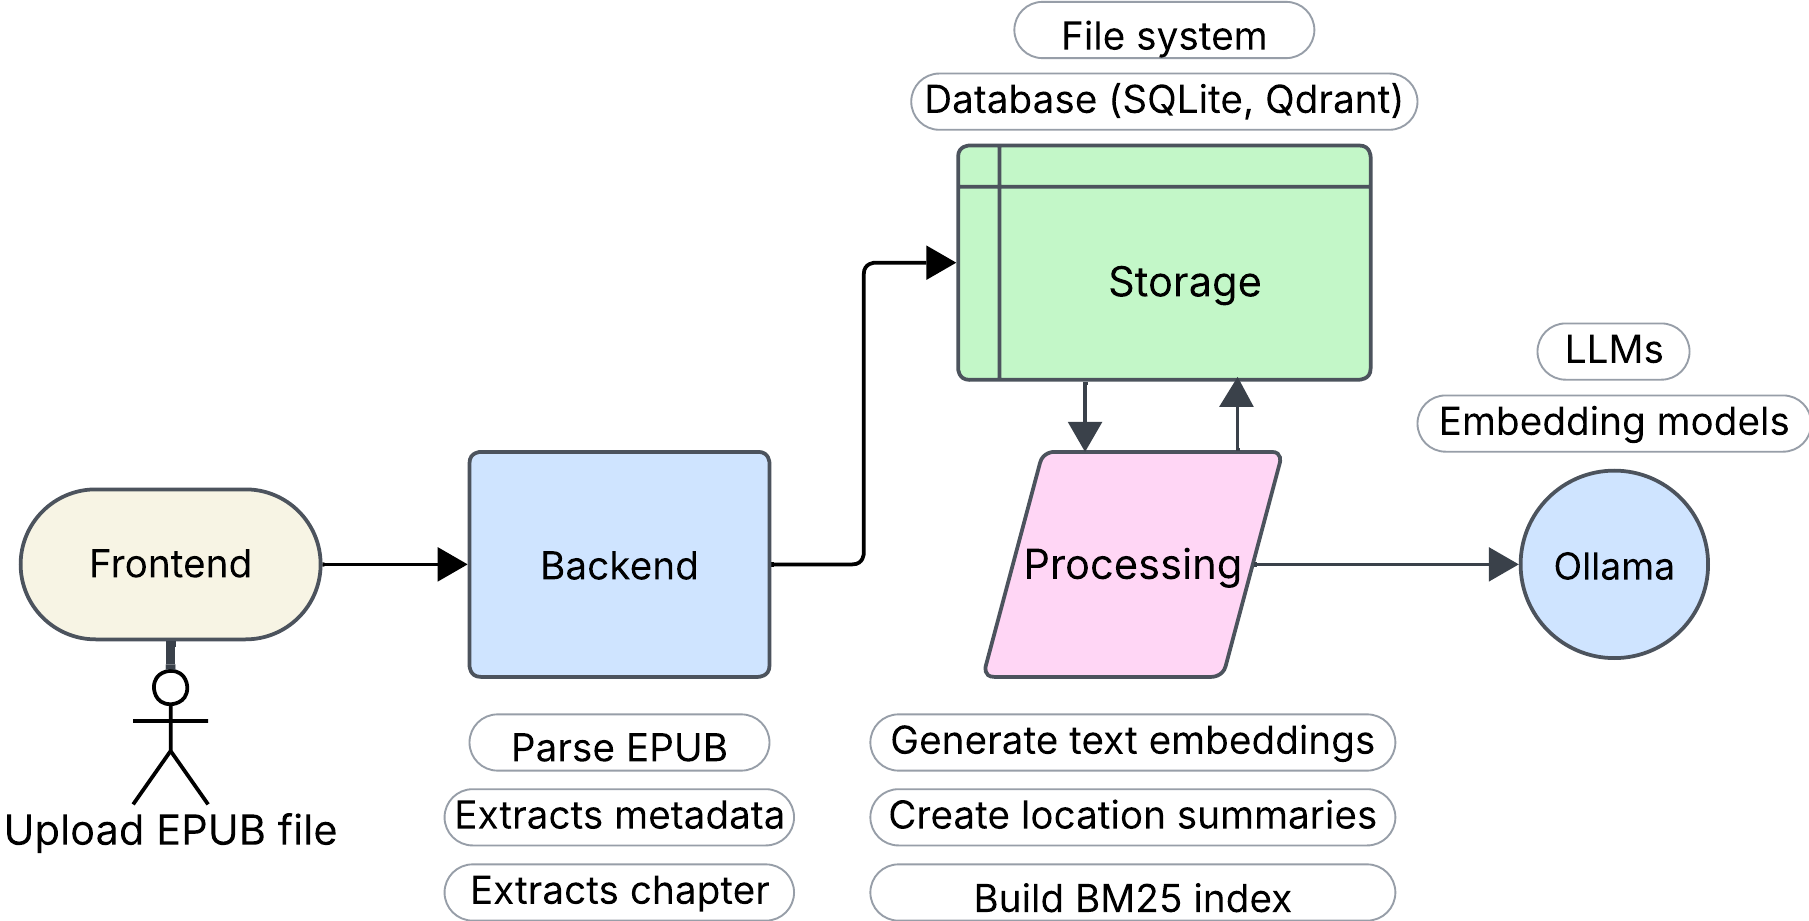
\includegraphics[width=0.55\linewidth]{images/hla_v2.png}
  \caption{High Level Architecture}
  \label{fig:hla}
\end{figure}

% \begin{figure}[!htbp]
%   \centering
%   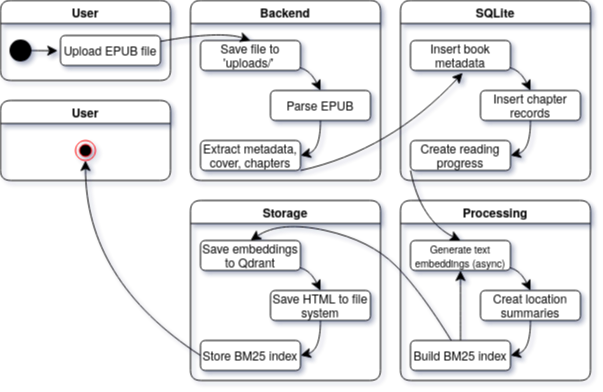
\includegraphics[width=0.95\linewidth]{images/information_flow.png}
%   \caption{Information Flow}
%   \label{fig:information_flow}
% \end{figure}

The architecture, as shown in Figure~\ref{fig:hla}, is structured to promote clarity, with emphasis on maintaining distinct boundaries between components, thereby supporting modularity and ease of maintenance. The frontend of MeReader is developed using Tauri and Vue.js/JavaScript, leveraging a modular component structure to ensure a responsive and dynamic user experience. Each component is designed to handle a specific aspect of the user interface or interaction logic. The backend of MeReader is implemented using Python with FastAPI, providing a set of RESTful API endpoints that support the application’s core functionalities.
The backend is organized into specialized services, each responsible for distinct aspects of data processing, content management, and AI-driven features. 

MeReader utilizes a variety of storage solutions tailored to the specific needs of different data types within the system.
Each storage component is selected to optimize performance, reliability, and scalability for its designated role. Figure~\ref{fig:hla} also shows the journey of a book when it's first uploaded via the reader.
When a user uploads an EPUB file, (1) the original file is saved in a folder, (2) metadata is extracted, (3) content is processed and organized into chapters, (4) database records are created for the book and its structure, (5) text chunks are embedded and stored in the vector database and finally (6) content is made available for reading and querying.

\begin{figure}[!t]
  \centering
  \begin{minipage}[t]{0.48\columnwidth}
    \centering
    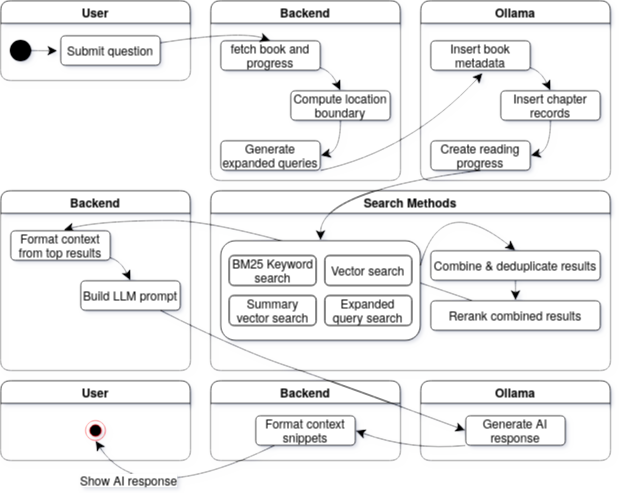
\includegraphics[width=\linewidth]{images/ai_query_flow.png}
    \caption{AI Query Flow}
    \label{fig:ai_flow}
  \end{minipage}\hfill
  \begin{minipage}[t]{0.48\columnwidth}
    \centering
    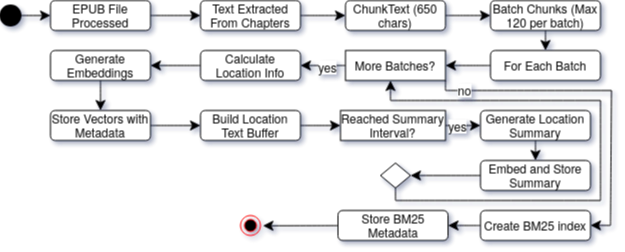
\includegraphics[width=\linewidth]{images/embedding_pipeline.png}
    \caption{Embedding Pipeline}
    \label{fig:embedding_pipeline}
  \end{minipage}
\end{figure}

Figure~\ref{fig:ai_flow} depicts the end-to-end workflow for processing an AI query within MeReader. Upon query initiation, the system first retrieves the relevant book together with the user’s current reading position. To ensure contextual focus, a location boundary is then applied, restricting the search space to the most relevant sections of the text. Within this scope, multiple retrieval techniques are executed in parallel, including vector search, BM25 keyword search~\cite{b28}, and query expansion. The outputs of these methods are subsequently consolidated, with duplicates removed and results reranked. The highest-ranked passages are assembled into a contextual block, which is combined with the original query to construct the final prompt. This prompt is submitted to the LLM, whose response is returned to the user alongside the contextual information.

The embedding pipeline, as shown in Figure~\ref{fig:embedding_pipeline}, converts a given book text into vector representations for semantic search. Important steps include optimal chunking, metadata storing and batched processing, all of which elevate the quality of said embedding. Text flows through sequential processing stages: content extraction, chunking, batch organization, embedding generation, and vector storage. The pipeline also generates summary embeddings at regular intervals to enable higher-level content understanding and builds BM25 indices alongside vector embeddings to support keyword-based search capabilities.